  %% diplomarbeit.tex
  %% Copyright 2015 Simon M. Laube
  %
  % This work may be distributed and/or modified under the
  % conditions of the LaTeX Project Public License, either version 1.3
  % of this license or (at your option) any later version.
  % The latest version of this license is in
  %   http://www.latex-project.org/lppl.txt
  % and version 1.3 or later is part of all distributions of LaTeX
  % version 2005/12/01 or later.
  %
  % This work has the LPPL maintenance status `author maintained'.
  % 
  % The Current Maintainer of this work is S. M. Laube
  %
  % This work consists of the files listed in ./Help/files.txt

%%=====================================================%%
%% Neues Diplomarbeitstemplate der ET	   			   %%
%% Abteilung ab 2013/2014				   			   %%
%% Erstellt von Simon Michael Laube		   			   %%
%% Betreut von  Prof. Mag. Dipl.-Ing. Dr. Daniel Asch  %%
%%			    Prof. Dipl.-Ing. Dr. Wilhelm Haager	   %%
%%=====================================================%%
%% Dokumentklasse KOMA-Script Report

%% benötigt, da scrpage2 mit KOMA-Script 3.3 (April 2020) entfernt wurde
%% Philipp Eilmsteiner 17.09.2020
\RequirePackage{scrlfile}
\ReplacePackage{scrpage2}{scrlayer-scrpage}

\documentclass[paper=a4,12pt]{scrreprt}
% Encoding UTF8
\usepackage[utf8]{inputenc}
% 8 Bit Aufloesung der Buchstaben
\usepackage[T1]{fontenc}
% Seitenraender
\usepackage[scale=0.72]{geometry}
% Spracheinstellungen
\usepackage[english, naustrian]{babel} % your native language must be the last one!!
% erweiterte Farbenpalette
\usepackage[dvipsnames]{xcolor}
% Abbildungen
\usepackage{graphicx}
% Tabellen (erweitert)
\usepackage{tabularx}
% TikZ + Circuit-TikZ (fuer Schaltungen)									
\usepackage[europeanresistors,							
			europeaninductors]{circuitikz}
% Nuetzliche TikZ Libraries
\usetikzlibrary{arrows,automata,positioning}
% Mathematikpakete!
\usepackage{amsmath,amssymb}							
%\usepackage{mathtools}	
% PDF Einbindung (zB Datenblaetter)
\usepackage{pdfpages}
% Source Code Einbindung, Setup siehe:
% http://en.wikibooks.org/wiki/LaTeX/Source_Code_Listings									
\usepackage{listings,scrhack} %scrhack vermeidet Umschaltung auf KOMA Floats..			
			
\usepackage{eurosym}
\usepackage{lscape}
% Diplomarbeitsspezifisches Package etdipa
\usepackage{etdipa}

%% Abkuerzungsverzeichnis
\usepackage[]{acronym}

%% Todos
\usepackage[]{todonotes}

%% Ganttdiagramme
\usepackage{pgfgantt}

%% Subfigures
\usepackage[lofdepth]{subfig}

%% HTL-Package (für HTL-Grün)
\usepackage{htlstp}

\usepackage{import}

\usepackage{array}
\usepackage{ragged2e}
\usepackage{csvsimple}
\usepackage{tikz}

%%==== Definitionen fuer die Diplomarbeit ============%%
\dokumenttyp{DIPLOMARBEIT}
\title{Luftkissenboot}
\author{Stefan Deimel \and Philipp Eilmsteiner \and Julia Stöger}
\date{\today}
\place{St. P\"olten}
\schuljahr{2020/21}
\professor{Dipl.-Ing. Helge Frank}
\dipacolor{htlgruen}
%%====================================================%%


% Hyperlinks im Dokument
\usepackage[colorlinks=true,
			linkcolor=black,
			citecolor=green,
			bookmarks=true,
			urlcolor=black,
			bookmarksopen=true]{hyperref}

\begin{document}

\listoftodos

\frontmatter

%%================ Titelseite ==========================%%
\maketitle
% Verantwortliche/Verfasser
\responsible{Stefan Deimel, Philipp Eilmsteiner, Julia Stöger}
%%======================================================%%


%%================ Eidesstattliche Erklaerung ==========%%
\begin{Eid}%Unterschrift der Diplomanden hinzufuegen!
\unterschrift{Stefan Deimel}
\unterschrift{Philipp Eilmsteiner}
\unterschrift{Julia Stöger}
\end{Eid}\newpage
%%======================================================%%

%%================ Diplomandenvorstellung ==============%%
%% start of file diplomanden.tex

%% Diplomandenvorstellung:
\begin{Diplomandenvorstellung}

\diplomand{Stefan Deimel}
		  {26.03.2002 in Tulln}
		  {Josef-Mohnl-Gasse 8}
		  {3435 Zwentendorf}
		  {\schule{2015--2021}{HTBLuVA St.Pölten, Abteilung für Elektrotechnik}
		  \schule{2010--2015}{Gymnasium Tulln}}
		  {stefan.deimel@aon.at}
		  {Images/bild}
\newpage	  

\diplomand{Philipp Eilmsteiner}
		  {24.03.2002 in Scheibbs}
		  {Josef-Pfeiffer Straße 3}
		  {3250 Wieselburg}
		  {\schule{2015--2021}{HTBLuVA St.Pölten, Abteilung für Elektrotechnik}
		  \schule{2010--2015}{Gymnasium Wieselburg}}
		  {philipp.eilmsteiner@outlook.at}
		  {Images/bild}
\newpage

\diplomand{Julia Stöger}
		  {26.03.2002 in Tulln}
		  {Josef-Mohnl-Gasse 8}
		  {3435 Zwentendorf}
		  {\schule{2015--2021}{HTBLuVA St.Pölten, Abteilung für Elektrotechnik}
		  \schule{2010--2015}{Gymnasium Tulln}}
		  {stefan.deimel@aon.at}
		  {Images/bild}
		  
\end{Diplomandenvorstellung}

%% end of file diplomanden.tex

%%======================================================%%
\responsible{Stefan Deimel}


%%================ Danksagungen ========================%%
%% start of file danksagungen.tex

%% Danksagungen:
\begin{Danksagung}
    \responsible{Stefan Deimel, Philipp Eilmsteiner, Julia Stöger}
An dieser Stelle möchten wir uns bei all jenen bedanken, die uns bei unserer Diplomarbeit tatkräftig unterstützt und motiviert haben. \\

Zuerst bedanken wir uns recht herzlich bei Herrn Dipl.-Ing. Helge Frank, der uns während dieser Arbeit mit seinem Fachwissen unterstützt und weitergeholfen hat. 
Durch sein besonderes Interesse an dem Projekt gelang es ihm, sein Wissen sehr gut an uns zu übermitteln. \\

Weiters möchten wir uns bei Herrn Fachlehrer Meiseneder und bei Herrn Fachlehrer Binder für die großartige Unterstützung bei fehlendem Werkzeug und Fragen 
rund um das Thema Elektronik bedanken. Außerdem wollen wir auch allen anderen \\ Lehrerinnen und Lehrer danken, die uns mit ihrem Wissen weitergeholfen haben. \\

Spezieller Dank gilt auch unseren Familien, die uns stets motiviert haben und mental zur Seite gestanden sind. \\

Dank gebührt auch Herrn Ing. Andreas Bergen für seine tatkräftige Unterstützung und Ideen zu unserer Diplomarbeit. \\

Für die sehr gute Zusammenarbeit und die finanzielle Unterstützung bedanken wir uns bei all unseren Sponsoren: Schrack for Students, Schmied \&\ Fellmann, Kustec, EMC und Gottwald.\\
\end{Danksagung}
\newpage

%% end of file danksagungen.tex
%%======================================================%%

%% Kurzfassungen
\todo[]{add Kurzfassungen}
%\includepdf[pages={1-2}, scale=1,]{KurzfassungDADE.pdf}
%\includepdf[pages={1-2}, scale=1,]{KurzfassungDAEN.pdf}

%%================ Abstract /Zusammenfass. =============%%
%% start of file zusammenfassung.tex

\selectlanguage{naustrian}
\begin{abstract}
\responsible{Julia Stöger}
Das Ziel unserer Diplomarbeit ist es, aus einem Schlauchboot ein funktionstüchtiges elektrisches Luftkissenboot zu bauen, welches
sich sowohl am Land, als auch auf Wasser fortbewegen kann. 
Das Hovercraft hat 2 Motoren und zugehörige Propeller, einen für den Auftrieb, um den Schwebezustand zu erreichen, und einen für den Antrieb.  \\
Die Ansteuerung der beiden Motoren erfolgt über je ein Daumengas, welche an dem Lenker befestigt sind. \\
Der Aufbau auf dem Boot wurde aus Holz gebaut. Elektrische Komponenten, wie Motoren, Propeller und ähnliches wurden zugekauft. \\
Für das Aufladen der Akkumulatoren wird ein Ladegerät angeschlossen, sodass die Akkus nicht aus dem Hovercraft 
entfernt werden müssen. 
\end{abstract}

%% end of file zusammenfassung.tex
\todo[]{add zusammenfassung}
%% start of file abstract.tex

\selectlanguage{english}
\begin{abstract}
    \todo{update this}
The main aim of this diploma project is to convert a inflatable dinghy to an operative hovercraft, 
which is able to drive on land and water. The hovercraft has 2 motors and propellers, one for floating and the other 
one for the electric drive. \\
To control the motors we have two thumb throttles, which are attached to the handlebar. \\
The construction on the boat is made of wood. Electrical components, such as motors and propellers were 
purchased. \\
To charge the batteries a charger has to be plugged in, so that the accumulators are able to stay in the Hovercraft
during the whole charging process.  
\end{abstract}
\selectlanguage{naustrian}

%% end of file abstract.tex
\todo[]{add abstract}
%\selectlanguage{english} % necessary for English speaking users

% delete this line if your native language is German 
%%======================================================%%

%%================ Inhaltsverzeichnis ==================%%
\tableofcontents
%%======================================================%%


%Ab hier Hauptteil
\mainmatter
\def\chapterpagestyle{headings} 
\chapter{Einführung}
\responsible{Julia Stöger}
Aus einem Schlauchboot wurde mit Hilfe von zwei Elektromotoren ein voll funktiontüchtiges Luftkissenboot gebaut. \\
Dieses ist in der Lage, eine erwachsene Person mehrere Minuten, über dem Boden schwebend, zu befördern. \\


\todo[]{Einführung bissal ausformulieren}
\section{Funktionsprinzip eines Hovercrafts}
\responsible{Julia Stöger}
Die Grundlage für das Schweben des Luftkissenbootes ist der auf den Boden gerichtete Luftstrom. Die Luft wird vertikal stark nach unten geleitet, wo ein Luftpolster entsteht. 
Durch ein Loch im Boden des Hovercrafts kann die Luft entweichen und somit einen Druck erzeugen, um das Luftkissenboot zum Schweben zu bringen. \\
Mithilfe von Fahnen, welche hinter dem Propeller am Boot angebracht sind, lässt sich das Hovercraft lenken. Für eine vereinfachte Darstellung der Funktionsweise siehe 
\autoref{fig:Funktionsprinzip}.

\begin{figure}[H]
  \centering
  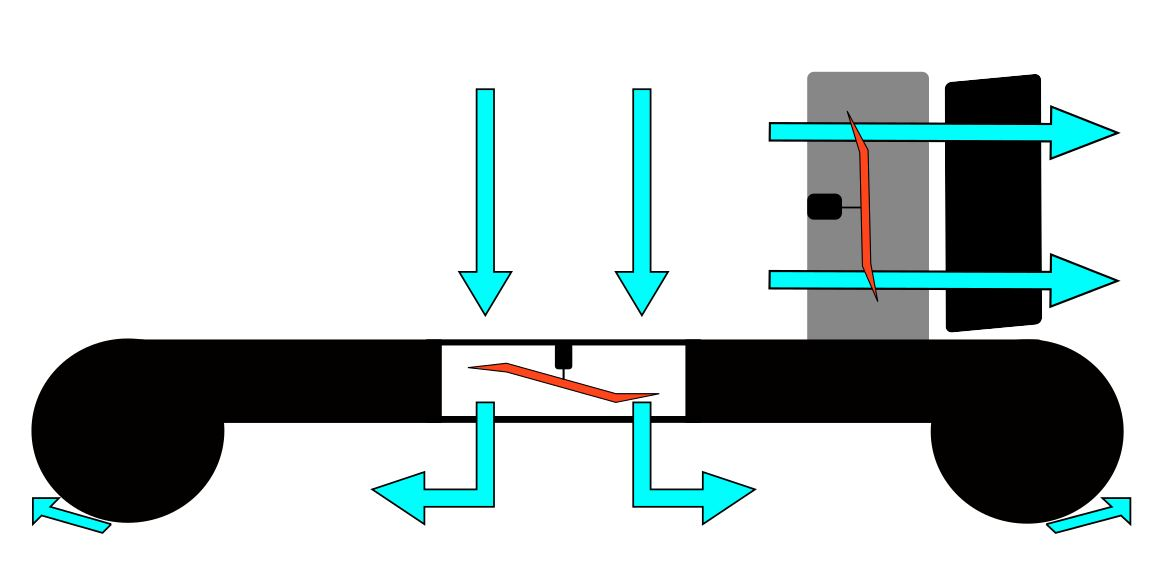
\includegraphics[width=\textwidth]{../Funktionsprinzip/Funktionsprinzip.JPG}
  \label{fig:Funktionsprinzip}
  \caption{Funktionsprinzip eines Hovercrafts}
\end{figure}


\section{Individuelle Themenstellung}

\begin{itemize}
  \item \textbf{Stefan Deimel:}
  \begin{itemize}
    \item Konstruktion
    \item Motorregelung
  \end{itemize}
  \item \textbf{Philipp Eilmsteiner:}
  \begin{itemize}
    \item Steuerelektronik
    \item HMI
  \end{itemize}
  \item \textbf{Julia Stöger:}
  \begin{itemize}
    \item Sicherheitskonzept
    \item Batteriemanagement
  \end{itemize}
\end{itemize}



\chapter{Erster Prototyp}
\responsible{Stefan Deimel}
\subimport{Textparts/Deimel/ErsterPrototyp/}{ErsterPrototyp.tex}

\chapter{Konstruktion}
\responsible{Stefan Deimel}
\subimport{Textparts/Deimel/Konstruktion/}{Konstruktion.tex}





\chapter{Meilensteine}
\responsible{Julia Stöger}
\subimport{Textparts/Stoeger/Meilensteine/}{Meilensteine.tex}

\chapter{Sicherheitskonzept}
\responsible{Julia Stöger}
\subimport{Textparts/Stoeger/Sicherheitskonzept}{Sicherheitskonzept.tex}

\chapter{Motoren \& Regler}
\responsible{Philipp Eilmsteiner}
\subimport{Textparts/Eilmsteiner}{Aktoren.tex}
\chapter{Boardelektronik}
\responsible{Philipp Eilmsteiner}
\subimport{Textparts/Eilmsteiner/Boardelektronik}{Boardelektronik.tex}

\clearpage
\appendix
\def\chapterpagestyle{empty} 

%%================ Abkuerzungsverzeichnis ==============%%
%% start of file abkuerzungen.tex

% Abkuerzungsverzeichnis
\addchap{
	\iflanguage{english}{Acronyms}{Abkürzungsverzeichnis}}
\begin{acronym}[ACRONYM]
\acro{tikz}[TikZ]{\TikZ{} ist kein Zeichenprogramm}
\acro{spi}[SPI]{Serial Peripheral Interface}
\acro{i2c}[I$^2$C]{Inter-Integrated Circuit}
\acro{xps}[XPS]{Extrudiertes Polystyrol}
\acro{can}[CAN-Bus]{Controller Area Network}
\end{acronym}\newpage

%% end of file abkuerzungen.tex
%%======================================================%%


%%================ Abbildungsverzeichnis ===============%%
\setcounter{lofdepth}{2}
\dipalistoffigures
%%======================================================%%

%%================ Tabellenverzeichnis  ================%%
\setcounter{lotdepth}{2}
\dipalistoftables
%%======================================================%%

%%================ Literaturverzeichnis ================%%
\newpage
%% start of file literatur.tex

%% Literaturverzeichnis:
\begin{Literatur}
% The TeXbook by D. E. Knuth
\bibitem[1]{TeXbook}{\textbf{Donald~E.~Knuth:} \emph{The \TeX{}book}. 1986, {\scshape Addison--Wesley} Verlag,\\
ISBN-13: 978-0-201-13447-6} 
%
\end{Literatur}

%% end of file literatur.tex

 
 
%%======================================================%%
\end{document}
